%% Placeholder for discussion of duality

%Below are notes for Nov 20
In optimization theory, duality or the duality principle is the principle that optimization problems may be viewed from either of two perspectives, that is, the primal problem or the dual problem.

Let's consider the primal problem formulated as follows,
\begin{align*}
	\min \quad&F_0(x) \\
	s.t. \quad&F_i(x)\leq 0, i = 1,...,m\\
	&h_i(x)= 0, i = 1,...,p
\end{align*}
Note that we do not have any assumptions of convexity here.

So the feasible set for this problem is
$$D = (\cap^m_{i=1}\text{dom}\ F_i)\cap(\cap^p_{i=1}\text{dom}\ h_i)$$ 
and the optimal value is $p^*$, optimal variable is $x^*$.

\begin{definition}[The Lagrangian Function]
	We define the Lagrangian function as follows,
	$$L(x,\lambda,\nu) := F_0(x) + \sum^m_{i=1}\lambda_i F_i(x) + \sum^p_{i=1}\nu_i h_i(x)$$
	where
	$$\lambda =
	\begin{bmatrix}
	\lambda_1\\
	\lambda_2\\
	\vdots\\
	\lambda_m
	\end{bmatrix},\
	\nu = 
	\begin{bmatrix}
	\nu_1\\
	\nu_2\\
	\vdots\\
	\nu_p
	\end{bmatrix}$$
	
	The pairs $(\lambda, \nu)$ are called the "Lagrange multipliers" or "dual variables", and the domain for the Lagrangian function is given by 
	$$\text{dom}\ L = D\times \reals^m \times \reals^p$$
\end{definition}

\begin{definition}[The "dual" function]
	The dual function $g(\cdot, \cdot)$ is defined as 
	\begin{equation*}
		g(\lambda, \nu) = \min_{x\in D}\quad L(x,\lambda,\nu)
	\end{equation*}
	
	Note: removes dependence on $x$.
\end{definition}


\begin{definition} The dual optimization problem is formulated as
	\begin{align*}
		\max_{\lambda, \nu} \quad&g(\lambda, \nu) \\
		s.t. \quad&\lambda \geq 0
	\end{align*}
	
	Note: $\nu_i$ are unconstrained, and we denote the optimal value for dual problem as $d^*$, optimal dual variables as $\lambda^*$ and $\nu^*$.
\end{definition}


\subsection{Duality theory}
The duality theory says that, \textbf{for most convex optimization problem}, we have $d^* = p^*$, that is, the primal optimum equals to the dual optimum.

Recall the problem formulations previously, the primal optimization problem is formulated as 
\begin{align*}
	\min \quad&F_0(x) \\
	s.t. \quad&F_i(x)\leq 0, \quad i = 1,\cdots,m \\
	&h_i(x)= 0, \quad i = 1,\cdots,p
\end{align*}
The Lagrange function is given by 
\begin{equation*}
	L(x,\lambda,\nu) = F_0(x) + \sum^m_{i=1}\lambda_i F_i(x) + \sum^p_{i=1}\nu_i h_i(x)
\end{equation*}

The dual function is given by
\begin{equation*}
	g(\lambda, \nu) = \min_{x\in D}\quad L(x,\lambda,\nu) 
\end{equation*}

So the dual optimization problem is formulated as 
\begin{align*}
	\max \quad&g(\lambda, \nu) \\
	s.t. \quad&\lambda \geq 0
\end{align*}



\vspace{0.3cm}
\noindent\textbf{A few observations}
\begin{enumerate}
	
	\item $g(\lambda, \nu)$ is concave in $(\lambda, \nu)$ for all $F_0,...,F_m$, $h_0,...,h_p$.
	
	\begin{proof}
		Recall that
		$$g(\lambda, \nu) =\min_{x\in D}[F_0(x) + \sum^m_{i=1}\lambda_iF_i(x) + \sum^p_{i=1}\nu_ih_i(x) ]$$
		
		First, notice that Lagrange function is an affine function in $(\lambda, \nu)$ so it is concave(of course it is convex at the same time). Secondly, note that the dual function is a pointwise infimum of a family of affine functions in $(\lambda, \nu)$, and thus $g(\lambda, \nu)$ is concave.
	\end{proof}
	
	\item For any primal feasible $x$ (i.e., $F_i(x)\leq 0, \forall i = [m]$, $h_i(x)= 0,\forall i = [p]$ and dual feasible $(\lambda, \nu)$ (i.e., $\lambda \geq 0$), we have
	$$g(\lambda, \nu)\leq F_0(x)$$
	for any tuple $(x, \lambda, \nu) \in \mathcal{C}\times \reals^m_+\times \reals^p$, where $\mathcal{C}$ is the feasible set of the primal problem (contains all feasible $x$).
	
	\begin{proof}
		Notice that, we have
		\begin{align*}
			F_0(x) &\geq F_0(x) + \sum^m_{i=1}\lambda_iF_i(x) + \sum^p_{i=1}\nu_ih_i(x)\\
			&\geq \min_{x\in D} [F_0(x) + \sum^m_{i=1}\lambda_iF_i(x) + \sum^p_{i=1}\nu_ih_i(x)] \\
			&= g(\lambda, \nu)
		\end{align*}
		where the first summation on r.h.s is negative due to $\lambda_i\geq 0$ and $F_i(x)\leq 0$, and the second summation equals to zero due to $h_i(x)=0$. 
		
		Thus the desired result can be obtained by the definition of $\min$ function and dual function.
	\end{proof}
	
	The point of greatest interest is $x^*$, where $p^* = F_0(x^*)$.
	
	Plug in to the above inequality, for all dual feasible $(\lambda, \nu)$ (i.e., for $\lambda \geq 0$), we have
	\begin{equation*}
		p^* = F_0(x^*) \geq g(\lambda, \nu)
	\end{equation*}
	
	Optimize over $(\lambda, \nu)$ where $\lambda \geq 0$ in order to maintain dual feasibility, we can get the greatest lower bound,
	\begin{equation*}
		p^* = F_0(x^*) \geq g(\lambda^*, \nu^*) = d^*
	\end{equation*}
	
	That is, we have the so called \textbf{weak duality}, $p^*\geq d^*$. 
	
	Furthermore, we refer to the difference $p^* - d^*$ as the \textbf{optimal duality gap}.
	
	
	\item For convex primal optimization problems, (i.e., $F_i(x)$ are convex and $h_i(x)$ are affine) and under certain conditions called "constraint qualification" (i.e., not all constraint sets allowed), the \textbf{strong duality} holds, i.e.,
	$$p^* = d^*$$
	and thus the optimal duality gap is zero.
	
	There are many types of constraint qualification, and we will introduce a simple one called Slater's condition in the next section.
	
\end{enumerate}
	

%Above are notes for Nov 20

% Below are notes for Nov 25
\subsection{Slater Conditions}

\begin{definition}[Slater conditions]
	Consider a primal problem with a set of constraints $F_i(x)\leq 0$, $i = [m]$ and $Ax = b$, it is said to be satisfied the Slater's conditions if there exists an $x\in\text{relint}\ D$ such that
	
	\begin{enumerate}
		\item $F_i(x) < 0,\ \forall i = [m]$
		
		\item $Ax = b$
	\end{enumerate}
	
	Furthermore, if some of the inequality contraints are defined by affine functions, this conditions can be weaken a bit. Suppose $F_i$ are affine for $i=1,\cdots, k$, where $k<m$, then the Slater conditions requires that there exists an $x\in\text{relint}\ D$ such that
	\begin{enumerate}
		\item $F_i(x) \leq 0,\ \forall i = 1,\cdots, k$
		\item $F_i(x) < 0,\ \forall i = k+1,\cdots, m$.
		\item $Ax = b$
	\end{enumerate}
	
\end{definition}

\begin{example}
	Convex problem that doesn't satisfy Slater's:
	\begin{align*}
		\begin{bmatrix}
			(x_1-1) & x_2
		\end{bmatrix}\begin{bmatrix}
			1&0\\
			0&1
		\end{bmatrix}\begin{bmatrix}
			x_1 - 1\\
			x_2
		\end{bmatrix}\leq 1\\
		\begin{bmatrix}
			(x_1+2) & x_2
		\end{bmatrix}\begin{bmatrix}
			1&0\\
			0&0
		\end{bmatrix}\begin{bmatrix}
			x_1 + 2\\
			x_2
		\end{bmatrix}\leq y
	\end{align*}
\end{example}

Feasible set is $(x_1, x_2) = \{(0,0) \}$

\begin{marginfigure}
	\centering
	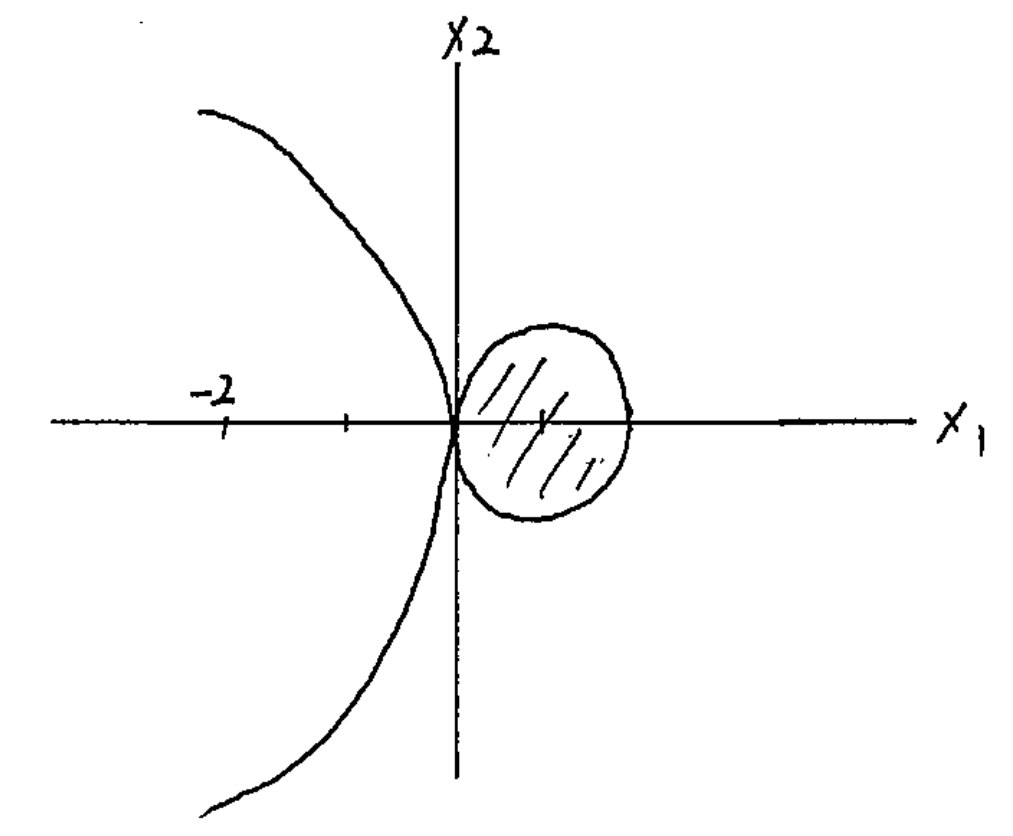
\includegraphics[width=1.8in,height=1.8in]{figures/ch10/figure1125_1.png}
	%\caption{This is an inserted JPG graphic} 
	%\label{fig:graph} 
\end{marginfigure}

\begin{theorem}
	If the primal optimization problem is convex and satisfies Slater's conditions, then $p^* = d^*$, the strong duality holds.
\end{theorem}

\begin{proof}

We propose a sketch proof for the case $m = 1$, i.e., 1 inequality constraint and there is no equality constraint so $p = 0$.

Given the basic setting for this case, the primal problem is given by
\begin{align*}
	\min \quad & F_0(x)\\
	s.t. \quad & F_1(x) \leq 0
\end{align*}
and we let $p^*$ be the optimal value of the primal problem.

The Lagrange function is:
$$L(x, \lambda) = F_0(x) + \lambda F_1(x)$$

The dual function is
$g(\lambda) = \min_{x\in D} L(x,\lambda) = \min_x{F_0(x) + \lambda F_1(x)}$

The dual optimal problem is formulated as
\begin{align*}
	\max \quad & g(\lambda)\\
	s.t. \quad & \lambda  \geq 0
\end{align*}
and we let $d^*$ be the optimal value of the dual problem.

To start, we define a set
\begin{align*}
	G 
	&= \{(F_1(x), F_0(x)) \vert x\in D = \text{dom}\ F_1\cap \text{dom}\ F_0 \}\\
	&= \cup_{x\in D}\{(F_1(x), F_0(x)) \}
\end{align*}

\begin{marginfigure}
	\centering
	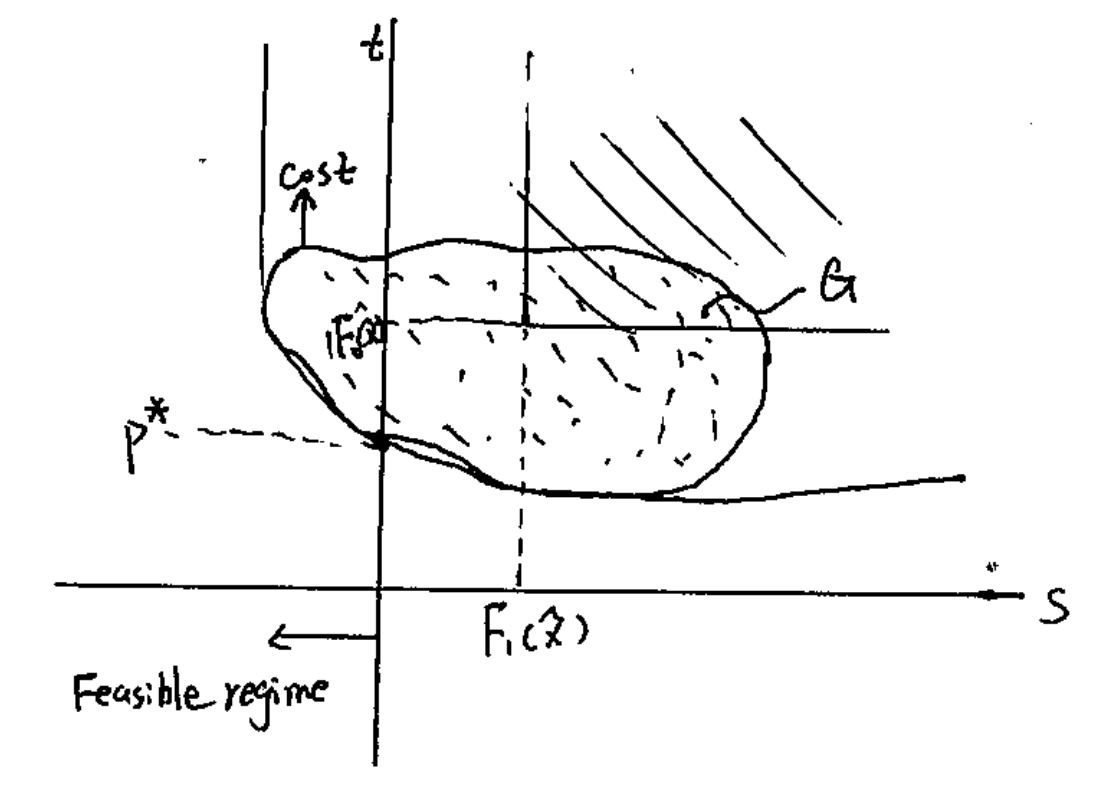
\includegraphics[width=1.8in,height=1.8in]{figures/ch10/figure1125_2.png}
	%\caption{This is an inserted JPG graphic} 
	%\label{fig:graph} 
\end{marginfigure}

and also define the set $\mathcal{A}$
\begin{align*}
	\mathcal{A} 
	&= G + \reals_+ \times \reals_+\\
	&= \{(s,t) \vert F_1(x)\leq s, F_0(x)\leq t, x\in D \}\\
	&= \cup_{x\in D}\{(s,t)\vert F_1(x)\leq s, F_0(x)\leq t \}
\end{align*}

A few observations regarding these two sets:
\begin{itemize}
	\item The set $G$ contains all information about primal problem.
	
	\item The set $\mathcal{A}$ contains all points "above" and to "right" of each point in $G$.
	
	\item Each such point(above and to right) is less interesting than the point in $G$ due to  
	
	(1) Perhaps higher cost
	
	(2) Perhaps more resources
\end{itemize}

The boundary of $\mathcal{A}$ is specified by the function:
\begin{align*}
	p(u) = &\min \quad F_0(x)\\
	&s.t. \quad F_1(x) \leq u
\end{align*}
($p$ is the boundary, $\mathcal{A}$ lies above the boundary)

A few observations regarding $p(u)$:

	(1) $p^* = p(0)$.
	
	(2) $p$ is non-increasing in $u$
	
	(3) $p$ is convex in $u$
	
	(4) $\mathcal{A} = \text{epi}\ p$

\begin{proof}[proof of (1)]
	When $u=0$, we just get the original primal problem so certainly $p^* = p(0)$.
\end{proof}

\begin{proof}[proof of (2)]
		As $u$ gets larger, feasible set of the $p(u)$ optimization gets larger so objective cannot increase $\rightarrow$ therefore non-increasing.
\end{proof}

\begin{proof}[proof of (3)]
	We want to prove the convexity of the problem
	\begin{align*}
		p(u) = &\min \quad F_0(x)\\
		&s.t. \quad F_1(x) \leq u
	\end{align*}
	
    and this means that we need to show $\forall u_1, u_2\in \text{dom}\ p$, $\forall \lambda\in [0,1]$, we have
	$$p(\lambda u_1 + (1-\lambda)u_2) \leq \lambda  p(u_1) + (1-\lambda)p(u_2).$$
	
	Consider $i=1, 2$, let
	\begin{align*}
		x_i = &\arg \min \quad F_0(x)\\
		&s.t. \quad F_1(x) \leq u_i
	\end{align*}
	
	That is, $F_0(x_1) = p(u_1)$ and $F_0(x_2) =p(u_2)$.
	
	Let $\tilde{x} = \lambda x_1 + (1-\lambda)x_2$, and note that
	 $$x_1\in \text{dom}\ F_1\cap \text{dom}\ F_0\cap \{x\vert F_1(x)\leq u_1 \}$$ $$x_2\in \text{dom}\ F_1\cap \text{dom}\ F_0\cap \{x\vert F_1(x)\leq u_2 \}$$
	
	So we can write
	\begin{align*}
		F_1(\tilde{x}) 
		&= F_1(\lambda x_1 + (1-\lambda)x_2)\\
		&\leq \lambda F_1(x_1) + (1-\lambda)F_1(x_2) \\
		&\leq \lambda u_1 + (1-\lambda)u_2
	\end{align*}
	where the first equality is due to $\tilde{x}\in \text{dom}\ F_1$, the first inequality is due to convexity of $F_1$, and the second inequality is due to $F_1(x_i) \leq u_i, i=1, 2.$
	
	Hence, 
	\begin{equation*}
		\tilde{x} \in \text{dom}\ F_1 \cap \text{dom}\ F_0 \cap \{x\vert F_1(x)\leq \lambda u_1 + (1-\lambda)u_2 \}
	\end{equation*}
	
	Therefore, $\tilde{x}$ is a feasible point for the optimization problem $p(\lambda u_1+(1-\lambda)u_2)$	
\end{proof}



Think about the trade-off between $F_1(x)$ and $F_0(x)$ in a slightly different way:
\begin{align*}
	\min_{(s,t)} \quad&\lambda s + t\\
	\text{where} \quad&(s,t) \in \mathcal{A}
\end{align*}
which is equivalent to
\begin{align*}
	\min_{(s,t)} \quad&\begin{bmatrix}
		\lambda &1 
	\end{bmatrix}\begin{bmatrix}
		s\\
		t
	\end{bmatrix}\\
	\text{where} \quad &(s,t) \in \mathcal{A}
\end{align*}

\begin{marginfigure}
	\centering
	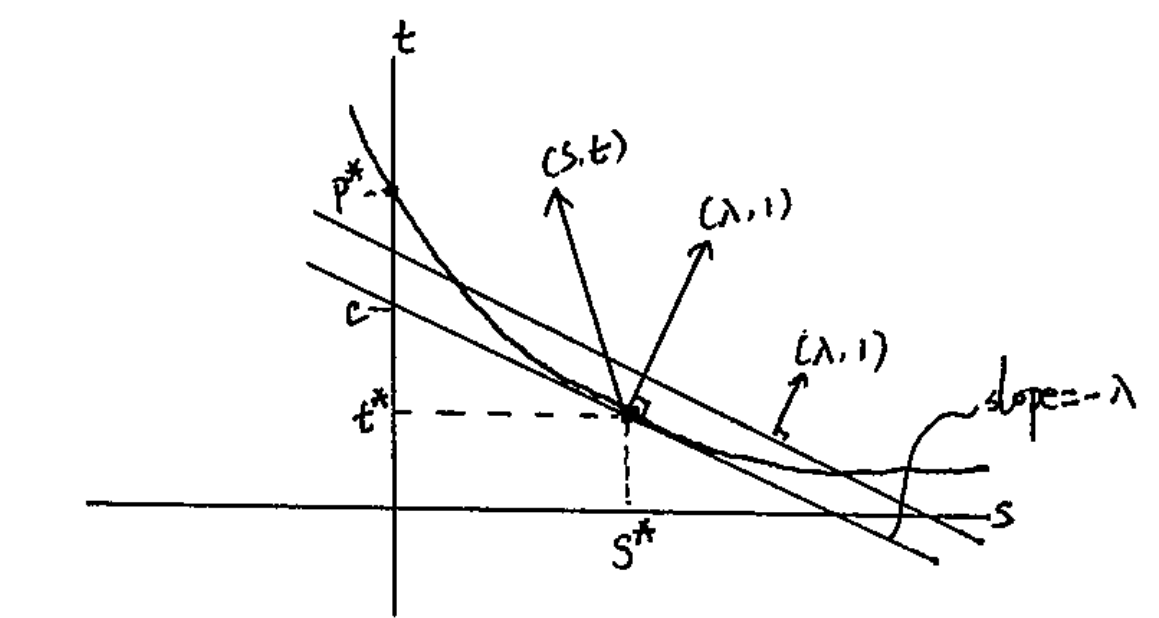
\includegraphics[width=1.8in,height=1.8in]{figures/ch10/figure1125_3.png}
	%\caption{This is an inserted JPG graphic} 
	%\label{fig:graph} 
\end{marginfigure}

For a given $\lambda$, the optimum is attained by some point $(s^*, t^*)$ on boundary of $\mathcal{A}$. Point on boundary is a function of $\lambda$, so we can write $$(s^*(\lambda), t^*(\lambda)) = (F_1(x^*(\lambda)), F_0(x^*(\lambda)))$$ 

Consider any point $(s,t)\in \mathcal{A}$:
\begin{align*}
	&
	\begin{bmatrix}
		\lambda &1
	\end{bmatrix}
	\begin{bmatrix}
		F_1(x^*(\lambda))\\
		F_0(x^*(\lambda))
	\end{bmatrix}
	\leq 
	\begin{bmatrix}
		\lambda &1
	\end{bmatrix}
	\begin{bmatrix}
		s\\
		t
	\end{bmatrix}\qquad  (*)\\
	\Leftrightarrow & 0\leq 
	\begin{bmatrix}
		\lambda & 1
	\end{bmatrix}
	\left(
	\begin{bmatrix}
		s\\
		t
	\end{bmatrix} 
	- 
	\begin{bmatrix}
		F_1(x^*(\lambda))\\
		F_0(x^*(\lambda))
	\end{bmatrix}\right)
\end{align*}

\begin{enumerate}
	\item This optimization yields a tangent plane, "supporting hyperplane"
	
	\item In this $2-D$ picture, supporting hyper-plane is a line, change $"\leq"$ in $(*)$ to $"="$ get a line 
	$$c =\lambda s + t$$
	where $c$ is the l.h.s of $(*)$.
	
	Rearrange yields $t = c - \lambda s$.
\end{enumerate}


This is the problem we just talked about:
\begin{align*}
	\min_{(s,t)\in \mathcal{A}} \quad \lambda s + t &= \lambda s^* + t^*\\
	&= \lambda F_1(x^*(\lambda)) + F_0(x^*(\lambda))\\
	&= \min_{x\in D} \quad[\lambda F_1(x) + F_0(x)]\\
	&= g(\lambda) 
\end{align*}
so it is the dual function.

Put these pieces all together:

	(1) The dual function $g(\lambda)$ specifies the $y-$intercept of the tangent line of slope $-\lambda$.
	
	(2) Last time proved $g(\lambda)$ is a lower bound on $p^*$ as long as $\lambda$ are dual-feasible (i.e., $\lambda \geq 0$).
	
	(3) The $y-$intercept is a lower bound on $p^*$, i.e., $c\leq p^{*}$.


Get best lower bound by maximizing $g(\lambda)$ over $\lambda \geq 0$, that is, solve the following optimization problem
\begin{align*}
	\max \quad &g(\lambda)\\
	s.t.\quad &\lambda \geq 0
\end{align*}
which exactly takes the form of dual problem.

\end{proof}


% Above are notes for Nov 25



% Below are notes for Nov 27

%\begin{align*}
%\max \quad &F_0(x)\\
%s.t. \quad&F_1(x) \leq 0\\
%\\
%L(x,\lambda) &= F_0(x) + \lambda F_1(x)\\
%g(\lambda) &= \min_{x\in D} L(x,\lambda)\\
%d^* &= \max \quad g(\lambda)\quad s.t.\quad \lambda \geq 0 
%\end{align*}
%
%\begin{equation*}
%\mathcal{A} =\{(s,t)\vert F_1(x)\leq s, F_0(x)\leq t, x\in D \}
%\end{equation*}
%
%
%\begin{marginfigure}
%\centering
%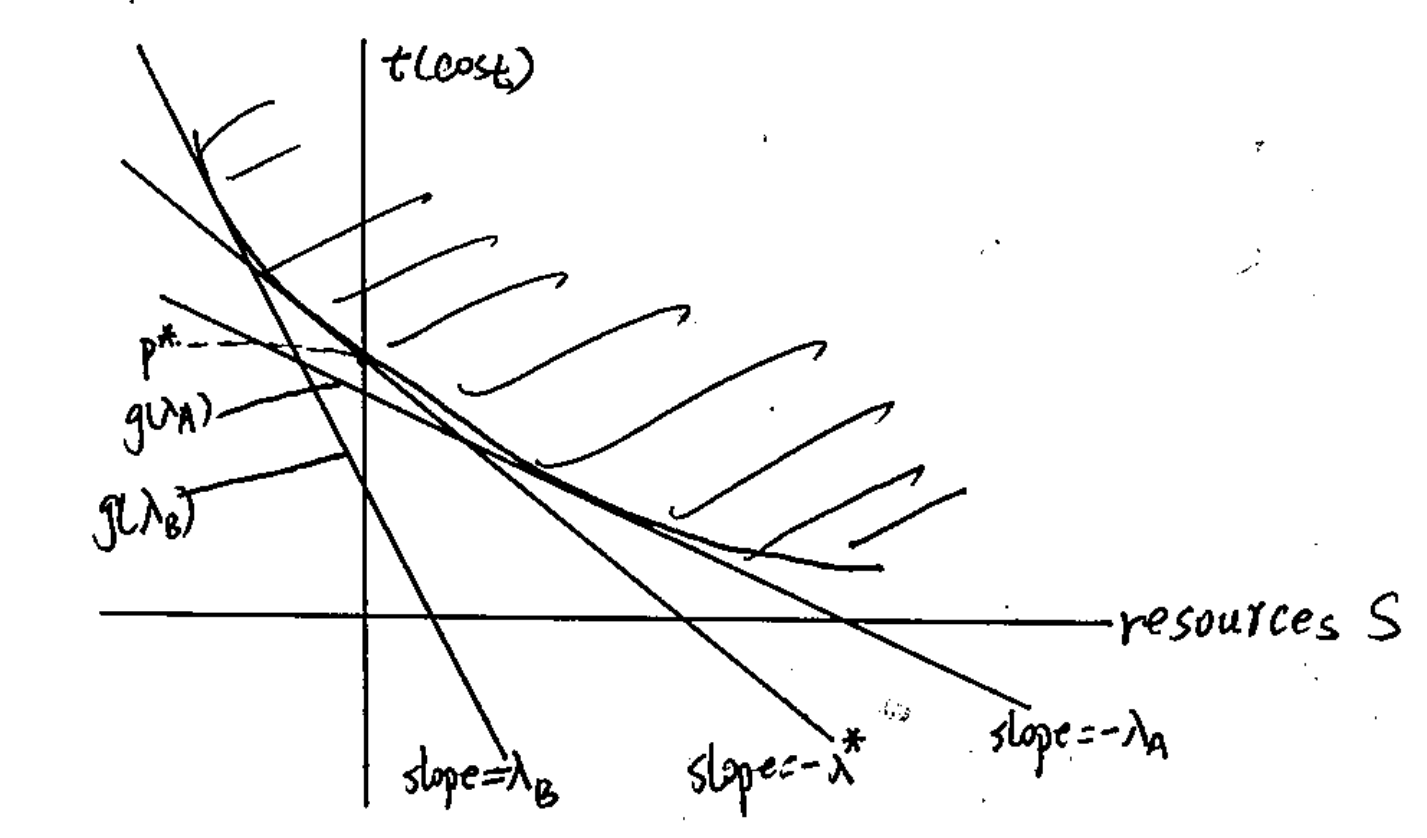
\includegraphics[width=1.8in,height=1.8in]{figures/ch10/figure1127_1.png}
%%\caption{This is an inserted JPG graphic} 
%%\label{fig:graph} 
%\end{marginfigure}


\vspace{0.3cm}
\subsection{"Pricing" Interpretation}
There is an interesting and intuitive interpretation for the duality theory called the pricing interpretation. Suppose the variable $x$ denotes how an company operates(i.e., "policy") and $F_0(x)$ denotes the cost of operating at policy $x$. Each constraint denotes representing some limit, such as a limit on resources, labor, etc. 

To optimal policy(i.e., $x^*$) with these constraints can be found by solving the problem(consider this is the primal problem)
\begin{align*}
	\min \quad & F_0(x)\\
	s.t.\quad & F_i(x) \leq 0,\quad i = 1,\cdots,m\\
	& h_i(x) = 0,\quad i = 1,\cdots,p
\end{align*}

In the next step, we reformulate this problem as an unconstrained problem by introducing $I$ and $\tilde{I}$, which are given by
\begin{equation}
I(x)=\left\{
\begin{aligned}
0 & , & x\leq 0 \\
\infty & , & x>0
\end{aligned}
\right.
\end{equation}

\begin{marginfigure}
	\centering
	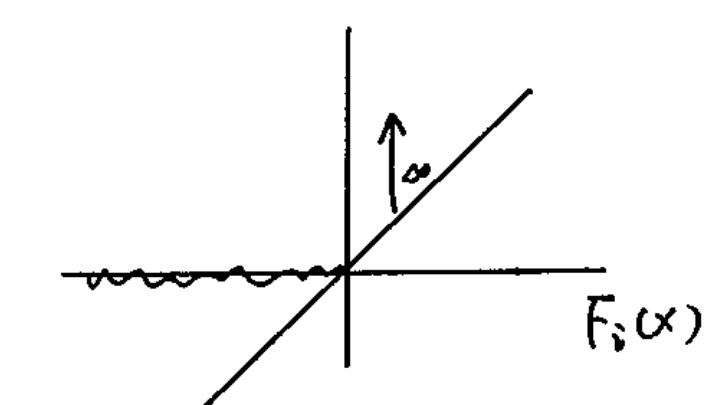
\includegraphics[width=1.8in,height=1.8in]{figures/ch10/figure1127_2.png}
	%\caption{This is an inserted JPG graphic} 
	%\label{fig:graph} 
\end{marginfigure}

\begin{equation}
\tilde{I}(x)=\left\{
\begin{aligned}
0 & , & x= 0 \\
\infty & , & \text{else}
\end{aligned}
\right.
\end{equation}


\begin{marginfigure}
	\centering
	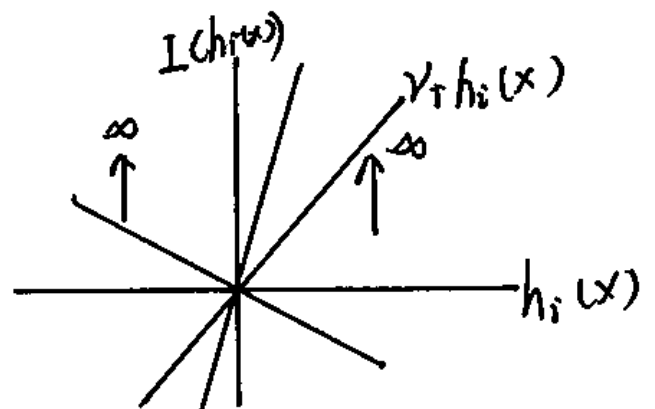
\includegraphics[width=1.8in,height=1.8in]{figures/ch10/figure1127_3.png}
	%\caption{This is an inserted JPG graphic} 
	%\label{fig:graph} 
\end{marginfigure}

So the primal problem can be reformulated as 
$$\min_x\quad F_0(x) + \sum^m_{i=1}I(F_i(x)) + \sum^p_{i=1}\tilde{I}(h_i(x)) \qquad (*)$$

This unconstrained problem is the same as primal one, but with "hard" penalties introducing by $I$ and $\tilde{I}$.

Now, let's consider the case that are more realistic. Suppose the company is allowed to break the limit on their resources by paying an additional cost which is linear in the amount of violation, measure by $F_i$ and $h_i$. More precisely, the additional payment made by the company for the $i$-th constraint is $\lambda_i F_i(x)$, and payments are also made to the company for the constraints that are not right(i.e., $F_i(x)<0$), the $\lambda_i F_i(x)$ represents a payment received by the company. 

So $\lambda_i$ is interpreted as the "price" for violating constraint $F_i$, and similarly we have $\mu_i$ as the "price" for violating constraint $h_i$.

Under this relaxed setting (i.e., not all constraints are satisfied), the problem can be formulated as 
$$F_0(x) + \sum^m_{i=1}\lambda_i F_i(x) + \sum^p_{i=1}\nu_i h_i(x)$$

It's obviously that such formulation takes the from of Lagrange function. If we minimize this function to obtain the minimal total cost and then maximize over $\lambda$ and $\nu$, that is
$$\max_{\lambda, \nu} \min_x F_0(x) + \sum^m_{i=1}\lambda_i F_i(x) + \sum^p_{i=1}\nu_i h_i(x)$$
where we obtain the optimal cost to the company under the least favorable set of prices. We use $d^*$ to denote this optimal value, and it readily follows that we have an interpretation for the weak duality, i.e.,
$$d^* \leq p^*$$


Furthermore, if strong duality holds, the problem $(*)$ (i.e., problem that is equivalent to the primal problem) becomes
\begin{align*}
	(*) 
	&= \max_{\lambda, \nu, \lambda \geq 0}\quad [\min_x\quad F_0(x) + \sum^m_{i=1}\lambda_iF_i(x) + \sum^p_{i=1}\nu_ih_i(x)]\\
	&= \max_{\lambda, \nu} g(\lambda, \nu) \quad \text{where}\ \lambda \geq 0
\end{align*}

Implication: Adjust the prices $\lambda, \nu$ so that the solution to relaxed problem matches the solution to the primal problem.
\subsection{Sensitivity Analysis}

\begin{marginfigure}
	\centering
	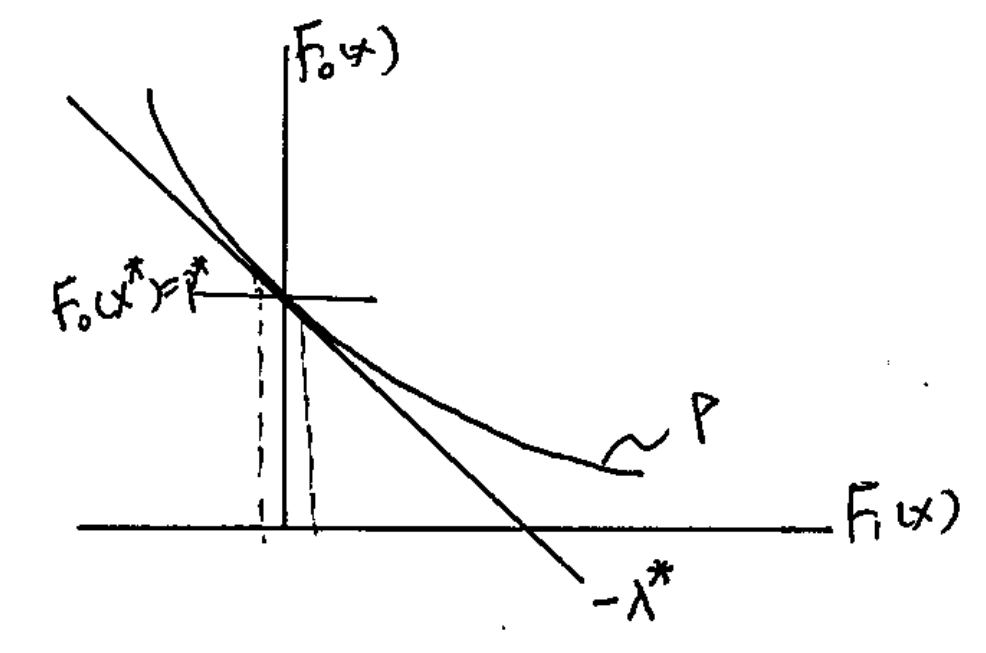
\includegraphics[width=1.8in,height=1.8in]{figures/ch10/figure1127_4.png}
	%\caption{This is an inserted JPG graphic} 
	%\label{fig:graph} 
\end{marginfigure}

\quad $\rightarrow$ At dual optimum slope of tangent is $-\lambda^*$

$\rightarrow$
If change constraint by $\epsilon$, optimum value will change by something like $(-\epsilon \lambda^*)$.


We consider the following perturbed version of the original optimization problem (unperturbed), says the perpetuated problem, as follows
\begin{align*}
	p^*(u,v) = \min \quad &F_0(x) \\
	s.t.\quad & F_i(x) \leq u_i ,\quad i = 1,\cdots,m\\
	& h_i(x) = v_i,\quad i = 1,\cdots, p
\end{align*}
where when $u=v=0$ is exactly the same as the unperturbed one.

$\rightarrow$ $u_i<0$ "tighten" constraint, $u_i>0$ loosen constraint, $v_i\neq 0$ change set-point.

$\rightarrow$ Same as $p(u)$ in last lecture.

$\rightarrow$ Note $p^*(0,0) = p^*$ is the optimal value of unperturbed problem.

$\rightarrow$ relate $p^*(u,v)$ to $p^*(0,0)$\\

\begin{itemize}
	\item Let $(\lambda^*, \nu^*)$ be optimal dual variables for unperturbed problem
	
	\item Consider a convex optimization problem satisfying Slater's conditions, i.e., strong duality holds,
	\begin{align*}
		p^*(0,0) &= g(\lambda^*, \nu^*)\\
		&= \min_{x\in D} L(x, \lambda^*, \nu^*)\\
		&\leq F_0(x) + \sum^m_{i=1}\lambda_i^* F_i(x) + \sum^p_{i=1}\nu_i^* h_i(x)\\
		&\leq F_0(x) + \sum^m_{i=1}\lambda_i^* u_i + \sum^p_{i=1}\nu^*_iv_i\\
		&= F_0(x) + (\lambda^*)^Tu+(\nu^*)^Tv
	\end{align*}
\end{itemize}
Our focus in on $x\in D$ s.t. $x$ is optimal for perturbed problem

i.e. $F_0(x)=p^*(u,v)$

$\Rightarrow$ $p^*(u,v) \geq p^*(0,0) - (\lambda^*)^Tu - (\nu^*)^Tv$

\begin{enumerate}
	\item E.g. If $\lambda_i >> 0$ and tighten constraint $F_i$ slightly so that $F_i(x)\leq -\epsilon < 0$
	$$p^*(u,v)\geq p^*(0,0) - (\lambda^*)^Tu - (\nu^*)^Tv$$
	
	\item Note not symmetric in general, big relaxation in constraint doesn't necessary mean big drop in cost.
	
	\item If $p(u,v)$ is differentiable, then have symmetry for small perturbations. 
\end{enumerate}

\subsection{Lagrange Method}
In order to solve the following primal problem,
\begin{align*}
	\min_x &\quad F_0(x)\\
	s.t. &\quad F_i(x) \leq 0,\quad i = 1,\cdots,m
\end{align*}
we propose the Lagrange method as follows:

	Step 1. First write Lagrangian: $L(x, \lambda) = F_0(x) + \sum^m_{i=1}\lambda_iF_i(x)$.
	
	Step 2. Solve for dual function $g(\lambda) = \min_{x\in D} L(x, \lambda)$, where $D$ is the primal feasible set.
	
	Step 3. Find $\lambda^* = \arg\max g(\lambda)$, s.t. $\lambda \geq 0$.
	
	Step 4. Recover the primal optimal $x^*$ by solving $\arg\min L(x, \lambda^*)$, that is, solve
		$$\arg\min F_0(x) + \sum^m_{i=1}\lambda_i^*F_i(x).$$

\noindent\textbf{Remarks:}
\begin{itemize}
	\item It is a nice approach if the problem has a nice structure, in particular if it is easy to solve for $(\lambda^*, \nu^*)$ analytically or numerically. 
	
	\item Even if the dual optimum $(\lambda^*, \nu^*)$ is unique, the primal optimum $x^*$ that minimized $L(x, \lambda^*, \nu^*)$ may not be unique.
\end{itemize}



\begin{example}[Lagrange Duality for LS problems]
	Consider the problem
	\begin{align*}
		\min_x \quad &\Vert x \Vert_2^2\\
		s.t.\quad &Ax = b
	\end{align*}
	where $x\in\reals^n$, $A\in\reals^{p\times n}$, $\rank(A) = p< n$.
	
	Recall the chapter least square, this an under determined LS problem, and the optimal solution is given by 
	$$x^* = A^T(AA^T)^{-1}b$$
	
	To verify that this solution is coincide with the one obtained by Lagrange's method, we proceed following procedure to solve this question.
	
	(1) Form the Lagrange function:
	 $$L(x, \nu) = x^Tx + \nu^T(Ax - b)$$
	
	(2) Solve for the dual function $g(\lambda) = \min_x L(x, \nu)$:
		
		Notice that Lagrange function here is a convex quadratic function of $x$(you may verify this), so simply by the first-order condition, we have
		$$\frac{\partial}{\partial x} L(x, \nu) = 2x+A^T\nu = 0\Rightarrow x^*(\nu) = -\frac{1}{2}A^T\nu$$

	(3) Find the dual optimum $\nu^*$:
	
	Now, we have dual problem as
	\begin{align*}
		\max_{\nu} g(\nu) &= \max_{\nu} L(x^*(\nu), \nu)\\
		&= \max_{\nu}[x^*(\nu)^Tx^*(\nu) + \nu^T(Ax^*(\nu) - b)]\\
		&= \max_{\nu}[\frac{1}{4}\nu^TAA^T\nu + \nu^T(A(-\frac{1}{2}A^T\nu)-b)]\\
		&= \max_{\nu}[\frac{1}{4}\nu^TAA^T\nu - \frac{1}{2}\nu^TAA^T\nu - \nu^Tb]\\
		&= \max_{\nu}[-\frac{1}{4}\nu^TAA^T\nu - \nu^Tb]
	\end{align*}
	
	Note that $g(\nu)$ is a concave quadratic function of $\nu$, and therefore utilize the first-order condition we yields
	\begin{align*}
	&\frac{\partial}{\partial \nu}(-\frac{1}{4}\nu^TAA^T\nu - \nu^Tb)= 0\\
	\Leftrightarrow&-\frac{1}{4} 2AA^T\nu - b = 0\\
	\Leftrightarrow& (AA^T)\nu = -2b\\
	\Leftrightarrow& \nu^* = -2(AA^T)^{-1}b
	\end{align*}

	(4) Substitute into $x^*(\nu)$ to get the primal optimum:
	\begin{align*}
	x^*(\nu^*) 
	&=-\frac{1}{2} A^T v^* \\
	&= -\frac{1}{2}A^T(-2(AA^T)^{-1}b)\\
	&= A^T(AA^T)^{-1}b
	\end{align*}

Hence, the optimal solution is coincide with our previous result in LS chapter, that is, for under-determined LS problem we have $x^* = A^T(AA^T)^{-1}b$.

Furthermore, at step (3), we have the problem
$$\max_{\nu} [- \frac{1}{4}\nu^TAA^T\nu - \nu^Tb ]$$

which is equivalent to 
$$\min_{\nu} [\frac{1}{4}\nu^TAA^T\nu + \nu^Tb ]$$

and it turns out, this minimization problem is equivalent to the following norm minimization problem,
\begin{align*}
\min_\nu\quad & \Vert\frac{1}{2}A^T\nu + x_0\Vert^2_2\\
s.t.\quad & Ax_0 = b 
\end{align*}
since they enjoy the same optimal solution $x^*$, and the difference of the optimal value is just a scalar.

More precisely, that's because
\begin{align*}
	\Vert \frac{1}{2}A^T\nu + x_0\Vert_2^2 
	&= (\frac{1}{2}A^T\nu+x_0)^T(\frac{1}{2}A^T\nu+x_0)\\
	&= \frac{1}{4}\nu^TAA^T\nu + 2\frac{1}{4}\nu^TAx_0 + x_0^Tx_0\\
	&= \frac{1}{4}\nu^TAA^T\nu + \nu^Tb+x_0^Tx_0
\end{align*}

\end{example}


\subsection{Final interpretation}
Consider the problem
\begin{align*}
	\min \quad & F_0(x)\\
	s.t. \quad & F_i(x)\leq 0\quad i = 1,\cdots,m
\end{align*}

We want connect to the problems with multiple (vector) objective $(F_0,F_1,\cdots,F_m)$, and one approach is to "scalarize" the objective as 
\begin{equation*}
	F_0(x) + \lambda F_1(x) + \cdots + \lambda_mF_m(x) = F_0(x) + \sum^m_{i=1}\lambda_iF_i(x)
\end{equation*}

% Above are notes for Nov 27





% Below are notes for Dec 2
\vspace{0.5cm}
\subsection{Dual of LPs}
Consider the primal problem is an LP problem as follows,
\begin{align*}
\min\quad &c^Tx\\
s.t.\quad &Ax\leq b
\end{align*}

The Lagrange function is 
\begin{align*}
L(x,\lambda) &= c^Tx + \sum^m_{i=1}(a_i^Tx-b_i)\\
&= c^Tx+\begin{bmatrix}
\lambda_1&\lambda_2&\cdots&\lambda_m
\end{bmatrix}\begin{bmatrix}
a_i^Tx-b_1\\
\vdots\\
a_m^Tx-b_m
\end{bmatrix} \\
&=c^Tx+\lambda^T(Ax-b)\\
&= -\lambda^Tb-(c^T+\lambda^TA)x
\end{align*}

The dual function is
\begin{align*}
g(\lambda) &= \min_x[-\lambda^Tb+(c^T+\lambda^TA)x]\\
&=
\label{eq6}
\left\{
\begin{aligned}
-\lambda^Tb &\quad \text{if} & c^T+\lambda^TA=0 \\
-\infty &\quad \text{if} & c^T+\lambda^TA\neq 0
\end{aligned}
\right.
\end{align*}

So the dual optimization problem is formulated as
\begin{align*}
\min\quad &g(\lambda)\\
s.t.\quad &\lambda \geq 0
\end{align*}

$\Rightarrow$
\begin{align*}
\min\quad &g(\lambda)\\
s.t.\quad &\lambda\geq 0\\
&c^T+\lambda^TA=0
\end{align*}

$\Leftrightarrow$
\begin{align*}
\min\quad &-\lambda^Tb\\
s.t.\quad &\lambda\geq 0\\
&c^T+\lambda^TA=0
\end{align*}





Following is initial note on Dec 2nd.

\begin{itemize}
	\item Dual of an LP is an LP
	
	\item Maybe not clear from form but have strong duality so $p^*=d^*$.
\end{itemize}

\begin{center}
\begin{tabular}{|c|c|c|}
	\hline 
	&Primal & Dual\\
	\hline  
	variables & $n$ & $m$\\
	\hline 
	constant&$m$&$n+m$\\
	\hline 
\end{tabular}
\end{center}


\begin{align*}
\min\quad &b^T\lambda\\
s.t.\quad &-\lambda\leq 0\quad\text{inequality multipliers }z\\
&A^T\lambda = -c\quad \text{equality multipliers }y
\end{align*}

\begin{align*}
L(\lambda,x,y) &= b^T\lambda + z^T(-\lambda)+y^T(A^T\lambda + c)\\
g(z,y) = \min_{\lambda}L(\lambda,z,y) &= \min_{\lambda}y^Tc+[b^T-z^T+y^TA^T]\lambda\\
&=
%\label{eq6}
\left\{
\begin{aligned}
y^Tc &\quad \text{if} &b^T-z^T+y^TA^T=0 \\
-\infty &\quad \text{if} &else
\end{aligned}
\right.
\end{align*}




Dual optimization:
\begin{align*}
\max\quad &g(z,y)\\
s.t.\quad &z \geq 0
\end{align*}
$\Leftrightarrow$


\begin{align*}
\min\quad &y^Tc\\
s.t.\quad &b^T-z^T+y^TA^T=0\\
&z\geq 0
\end{align*}
constants:


\begin{align*}
b^T=y^TA^T &= z^T\\
z&\geq 0
\end{align*}

$\Leftrightarrow$

\begin{equation*}
b^T+y^TA^T \geq 0
\end{equation*}

Thus this problem can also be written as:
\begin{align*}
\max\quad &y^Tc\\
s.t.\quad &b+Ay \geq 0
\end{align*}

$\Leftrightarrow$
\begin{align*}
\max\quad &(-x)^Tc\\
s.t.\quad &b+A(-x) \geq 0
\end{align*}

$\Rightarrow$
\begin{align*}
\max\quad &c^Tx\\
s.t.\quad &Ax \leq b
\end{align*}

% Above are notes for Dec 2
